\section{总体设计}

\subsection{移动端设计}

\textbf{本 App 使用 Apple 原生 UIKit 框架,基于 Swift 和 Objective-C 两种语言开发,以 Swift 为主,Objective-C 为辅。}UIKit 框架提供了 iOS 或 Apple tvOS app 所需的基础架构。它提供了用于实施界面的窗口和视图架构,用于向 app 提供多点触控和其他类型输入的事件处理基础架构,以及管理用户、系统和 app 之间互动所需的主运行循环。该框架提供的其他功能包括动画支持、文档支持、绘图和打印支持、当前设备的相关信息、文本管理和显示、搜索支持、辅助功能支持、app 扩展支持和资源管理 \footnote{https://developer.apple.com/documentation/uikit} 。在项目中,我们采用 \textbf{MVC 设计模式},即模型对(Model),视图对象(View)和控制器对象(Controller)。模型对象用于封装与应用程序的业务逻辑相关的数据以及对数据的处理方法。其不依赖控制器和视图,但模型的数据发生变化时,会通过一些机制实现在视图上的刷新,如观察者模式(KVO)等。视图对象能够实现数据有目的的显示,在视图中一般没有程序上的逻辑,而是由控制器进行管理。控制器对象起到不同层面间的组织作用,用于控制应用程序的流程。它处理事件并作出响应,包括用户的操作,数据模型的改变等。同时,由于传统 MVC 模式中网络操作难以合理安放,易造成控制器过厚等问题,我们将网络操作封装成了一个\textbf{单例类},易于复用,并且能减少控制器中网络操作的代码量。在单例模式(Singleton)中,一个单例类在整个程序中有且仅有一个实例化对象,并提供一个类方法供全局调用。

\begin{figure}[H]
    \centering
    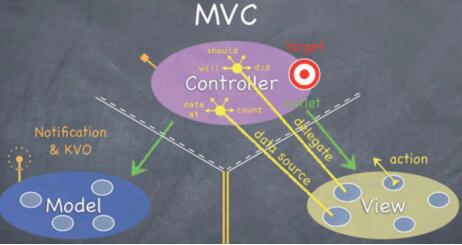
\includegraphics[width=0.8\textwidth]{figures/MVC.jpg}
    \caption{MVC模式示意图}
    \label{fig:my_label}
\end{figure}


由于我们使用原生 UIKit 框架,可以\textbf{同时开发适配 iPhone 和 iPad 应用}。同时,\textbf{借助 Mac Catalyst 框架}也可以将代码移植到 macOS 平台,\textbf{实现了 iOS、iPadOS 和 macOS 的三平台开发}。考虑到 Mac 平台强大的计算能力以及\textbf{高效的 ML Compute 框架},后期可以考虑为 Mac 版应用提供本地运行的风格迁移功能。

\subsection{服务器端设计}

由于 Python 语言在 ML 方面的优势,本 App 服务端使用 Python 后端框架 FastAPI 编写,该框架速度媲美 NodeJS 和 GO,吸取了 Django,Flask 等众多前辈的经验,非常适合构建后端 API。\textbf{同时该框架提供了协程异步的请求处理机制,因此后端 API 采用协程并行的方式进行构建,在多并发请求下具有较大的优势。}


\begin{figure}[H]
    \centering
    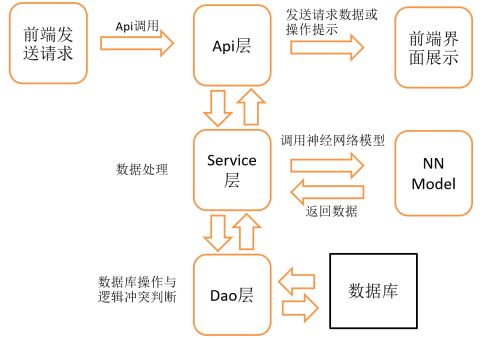
\includegraphics[width=0.8\textwidth]{figures/后端逻辑.png}
    \caption{后端逻辑示意图}
    \label{fig:my_label}
\end{figure}

后端的请求处理流程如上图所示,前端发送请求调用 API,后端在 API 层处理传入的请求并将响应发送回调用者。根据传入的请求调用 Service 层所需的服务程序或进行数据处理等,对于用户发帖、收藏等请求,服务程序与 Dao 层进行交互而操作数据库,对于音乐或图像艺术加工等请求,则需调用后端部署的神经网络模型。对于图像迁移模型,我们使用的是较为简单的 VGG-19 并达到了不错的效果;对于音乐迁移模型,该模型十分复杂,我们参考 Facebook 以及 OpenAI 等组织开源的音乐迁移模型,并根据我们的需求进行了调整和修改。
